% This file was created by matplotlib2tikz v0.7.4.
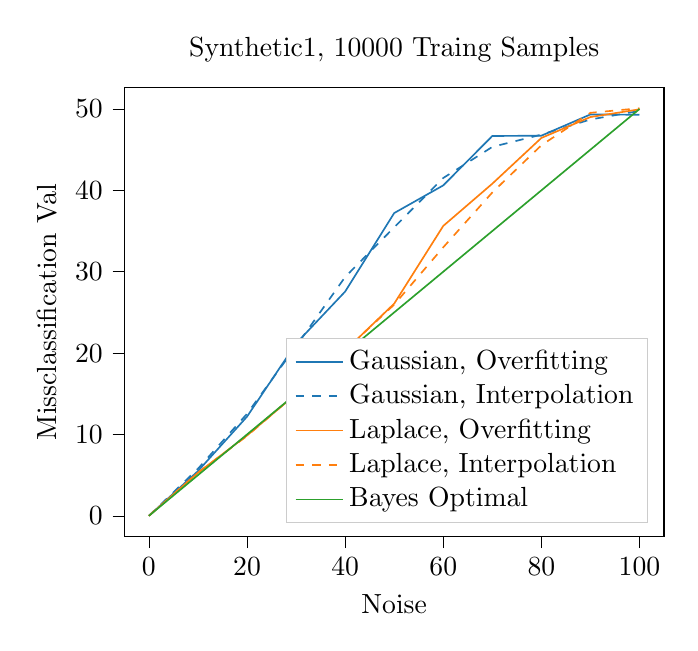
\begin{tikzpicture}

\definecolor{color0}{rgb}{0.12156862745098,0.466666666666667,0.705882352941177}
\definecolor{color1}{rgb}{1,0.498039215686275,0.0549019607843137}
\definecolor{color2}{rgb}{0.172549019607843,0.627450980392157,0.172549019607843}

\begin{axis}[
legend cell align={left},
legend style={at={(0.97,0.03)}, anchor=south east, draw=white!80.0!black},
tick align=outside,
tick pos=left,
title={Synthetic1, 10000 Traing Samples},
x grid style={white!69.01960784313725!black},
xlabel={Noise},
xmin=-5, xmax=105,
xtick style={color=black},
y grid style={white!69.01960784313725!black},
ylabel={Missclassification Val},
ymin=-2.5045, ymax=52.5945,
ytick style={color=black}
]
\addplot [semithick, color0]
table {%
0 0
10 5.50000000000001
20 12.19
30 21.18
40 27.56
50 37.21
60 40.61
70 46.68
80 46.72
90 49.33
100 49.29
};
\addlegendentry{Gaussian, Overfitting}
\addplot [semithick, color0, dashed]
table {%
0 0
10 5.79
20 12.54
30 20.85
40 29.35
50 35.46
60 41.52
70 45.34
80 46.85
90 48.71
100 49.76
};
\addlegendentry{Gaussian, Interpolation}
\addplot [semithick, color1]
table {%
0 0
10 5.3
20 9.87
30 14.97
40 20.3
50 26.08
60 35.63
70 40.82
80 46.44
90 49.01
100 49.96
};
\addlegendentry{Laplace, Overfitting}
\addplot [semithick, color1, dashed]
table {%
0 0
10 5.3
20 9.82
30 15.01
40 20.34
50 25.96
60 33
70 39.74
80 45.54
90 49.53
100 50.09
};
\addlegendentry{Laplace, Interpolation}
\addplot [semithick, color2]
table {%
0 0
10 5
20 10
30 15
40 20
50 25
60 30
70 35
80 40
90 45
100 50
};
\addlegendentry{Bayes Optimal}
\end{axis}

\end{tikzpicture}